\documentclass[fullscreen=true, bookmarks=true, hyperref={pdfencoding=unicode}]{beamer}
\usepackage[utf8]{inputenc}                                % Кодировка
\usepackage[english,russian]{babel}                        % Переносы
\usepackage{xcolor}                                        % Работа с цветом
\usepackage{amsmath,amssymb,amsfonts}                      % Символы АМО
\usepackage{graphicx}                                      % Графика
\usepackage[labelsep=period]{caption}                      % Разделитель в подписях к рисункам и таблицам
\usepackage{hhline}                                        % Для верстки линий в таблицах
\usepackage{tikz}                                          % Для простых рисунков в документе
\usepackage{fancybox}                                      % Пакет для отрисовки рамок
\usepackage{verbatim}                                      % Для вставки кода в презентацию
\usepackage{animate}                                       % Для вставки видео в презентацию
\usepackage{xmpmulti}                                      % Для вставки gif в презентацию
\usepackage{multirow}
\usepackage{mathrsfs}

\usetikzlibrary{arrows, snakes, backgrounds}                 % Для отрисовки стрелок
\usetikzlibrary{positioning, fit, arrows.meta, shapes, calc}
% used to avoid putting the same thing several times...
% Command \empt{var1}{var2}
\newcommand{\empt}[2]{$#1^{\langle #2 \rangle}$}

\graphicspath{{images/}}                                   % Путь до рисунков
\setbeamertemplate{caption}[numbered]                      % Включение нумерации рисунков

\definecolor{links}{HTML}{2A1B81}                          % blue for url links
\hypersetup{colorlinks,linkcolor=,urlcolor=links}          % nothing for others

\usetheme{boxes}
\usecolortheme{crane}

\usepackage{pythonhighlight}

\newtheorem*{question}{Вопрос}

\title{Лекция 4. Карты Кохонена, автокодировщики, перенос обучения, генеративно-состязательные сети}
\author{Александр Юрьевич Авдюшенко}
\institute{МКН СПбГУ}
\date{10 марта 2022}
\titlegraphic{
\includegraphics[keepaspectratio,width=0.5\textwidth]{logo_fmkn.png}}

\begin{document}
%\unitlength=2mm

% выводим заглавие
\begin{frame}
\transdissolve[duration=0.2]
\titlepage
\end{frame}


\begin{frame}
  \frametitle{Пятиминутка}
  \begin{itemize}
    \item Перечислите недостатки сверточных нейронных сетей
    \item Выпишите формулу простейшей (vanilla) рекуррентной сети
    \item Какие фильтры (gates) есть в LSTM?
  \end{itemize}
\end{frame}


\begin{frame}
  \frametitle{Постановка задачи кластеризации}
  \framesubtitle{напоминание}

  {\bf Дано}:

   $X^\ell = \{x_1, \dots, x_\ell \}$ — обучающая выборка объектов $x_i \in \mathbb{R}^n$

   $\rho: X \times X \to [0, \infty)$ — функция расстояния между объектами

  {\bf Найти}:

  $Y$ — множество кластеров, например, задаваемых своими центрами $w_y \in \mathbb{R}^n$

  Пусть алгоритм кластеризации
  $$a(x) = \arg\min\limits_{y \in Y} \rho(x, w_y)$$
  <<Правило жёсткой конкуренции>> (WTA, Winner Takes All)

  {\bf Критерий}: среднее внутрикластерное расстояние

  $$ Q(w; X^\ell) = \sum\limits_{i=1}^\ell \rho^2(x_i, w_{a(x_i)}) \to \min\limits_{w_y: y \in Y}$$
\end{frame}


\begin{frame}
  \frametitle{Сеть Кохонена — двухслойная нейронная сеть}

  \begin{center}
    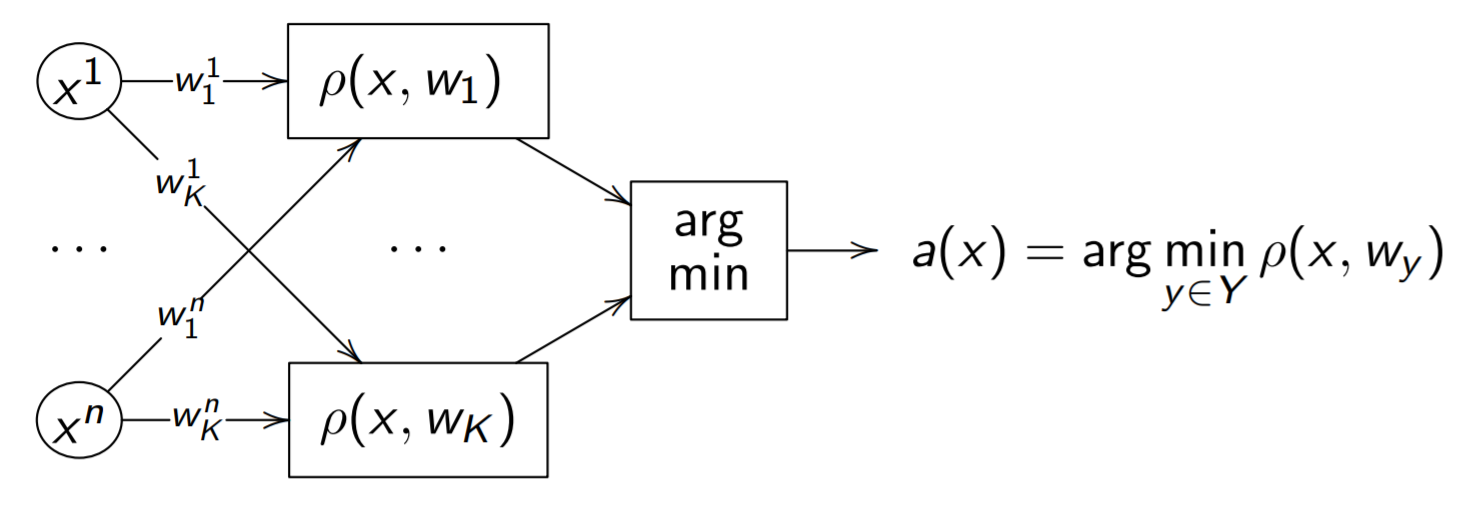
\includegraphics[keepaspectratio,
                     width=0.7\paperwidth]{kohonen-net.png}
  \end{center}

  Градиентный шаг в методе стохастического градиента:

  $$w_y = w_y + \eta(x_i-w_y)[a(x_i)=y]$$

  Если $x_i$ относится к кластеру $y$, то $w_y$ сдвигается в сторону $x_i$

  \noindent\rule{8cm}{0.4pt}

  {\it T. Kohonen.} Self-organized formation of topologically correct feature maps. 1982.
\end{frame}


\begin{frame}
  \frametitle{Стохастический градиентный спуск}

  {\bf Вход}: выборка $X^\ell$, темп обучения $\eta$, параметр $\lambda$

  {\bf Выход}: центры кластеров $w_1, \dots, w_K \in \mathbb{R}^n$

  \begin{enumerate}
    \item инициализировать центры $w_y,\ y \in Y$
    \item оценку функционала: $${Q} = \sum\limits_{i=1}^\ell \rho^2(x_i, w_{a(x_i)}) $$
    \item {\bf повторять}
      \begin{itemize}
        \item выбрать объект $x_i$ из $X^\ell$ (например, случайный)
        \item вычислить кластер: $y = \arg\min\limits_{y \in Y} \rho(x_i, w_y)$
        \item сделать градиентный шаг: $\color{red}{w_y = w_y + \eta (x_i - w_y)}$
        \item оценить функционал: ${Q} = \lambda \rho^2(x_i, w_y) + (1 - \lambda) {Q}$
      \end{itemize}
    \item {\bf пока} значение ${Q}$ и/или веса $w_y$ не сойдутся
  \end{enumerate}
\end{frame}


\begin{frame}
  \frametitle{Жесткая и мягкая конкуренция}

  {\bf Правило жёсткой конкуренции (WTA, Winner Takes All)}

  $$w_y = w_y + \eta(x_i-w_y)\color{red}{[a(x_i)=y]}, y \in Y$$

  {\bf Недостатки правила WTA}
  \begin{itemize}
    \item медленная скорость сходимости
    \item некоторые центры кластеров могут никогда не выбираться
  \end{itemize}

  {\bf Правило мягкой конкуренции (WTM, Winner Takes Most)}

  $$w_y = w_y + \eta(x_i-w_y)\color{red}{K(\rho\left(x_i, w_y)\right)}, y \in Y$$

  где ядро $K(\rho)$ — неотрицательная невозрастающая функция

  Теперь центры всех кластеров смещаются в сторону $x_i$, но чем дальше от $x_i$, тем меньше величина смещения
\end{frame}


\begin{frame}
  \frametitle{Карта Кохонена (Self Organizing Map, SOM)}

  Вводим прямоугольную сетку кластеров $\{1, \dots, SizeX\}\times \{1, \dots, SizeY\}$

  Каждому узлу $(x, y)$ приписан нейрон Кохонена $w_{xy} \in \mathbb{R}^n$

  Наряду с метрикой $\rho(x_i, w_{xy})$ вводится метрика на сетке:

  $$ r((x, y),(a, b)) = \sqrt{(x - a)^2 + (y - b)^2}$$

  \begin{center}
    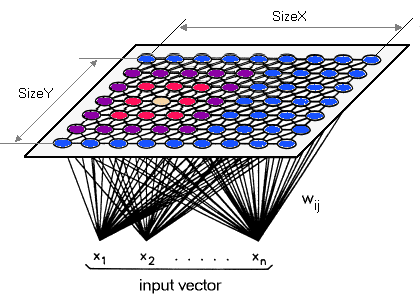
\includegraphics[keepaspectratio,
                     width=0.5\paperwidth]{kohonen-net-scheme.png}
  \end{center}
\end{frame}

\begin{frame}
  \frametitle{Обучение карты Кохонена}

  {\bf Вход}: выборка $X^\ell$, темп обучения $\eta$

  {\bf Выход}: $w_{xy} \in \mathbb{R}^n$ — векторы весов,

  \begin{enumerate}
    \item инициализировать веса: $w_{xy} = \text{random}\left(-\frac{1}{2MH}, \frac{1}{2MH} \right)$
    \item {\bf повторять}
    \begin{itemize}
      \item выбрать случайный объект $x_i$ из $X^\ell$
      \item WTA: вычислить координаты кластера: $$(a_i, b_i) = \arg\min\limits_{(a, b)} \rho(x_i, w_{ab})$$
      \item {\bf для всех} $(a, b) \in $ Окрестность $(a_i, b_i)$

       $\ \ \ $ WTM: сделать шаг градиентного спуска:

       $\ \ \ $ $w_{ab} = w_{ab} + \eta (x_i - w_{ab}) K(r((a_i, b_i), (a, b)))$
    \end{itemize}
    \item {\bf пока} кластеризация не стабилизируется
  \end{enumerate}
\end{frame}


\begin{frame}
  \frametitle{Интерпретация карт Кохонена}

  Два типа графиков — цветных карт $SizeX \times SizeY$

  \begin{itemize}
    \item Цвет узла $(a, b)$ — локальная плотность в точке $(a, b)$ — среднее расстояние до $k$ ближайших точек выборки
    \item По одной карте на каждый признак: цвет узла $(a, b)$ — значение $j$-й компоненты вектора $w_{ab}$
  \end{itemize}
  \vspace{1cm}
  Посмотрим на карты Кохонена, построенные на шести признаках, собранных у 1000 человек.
\end{frame}

{ % all template changes are local to this group.
    \setbeamertemplate{navigation symbols}{}
    \begin{frame}<article:0>[plain]
        \begin{tikzpicture}[remember picture,overlay]
            \node[at=(current page.center)] {
                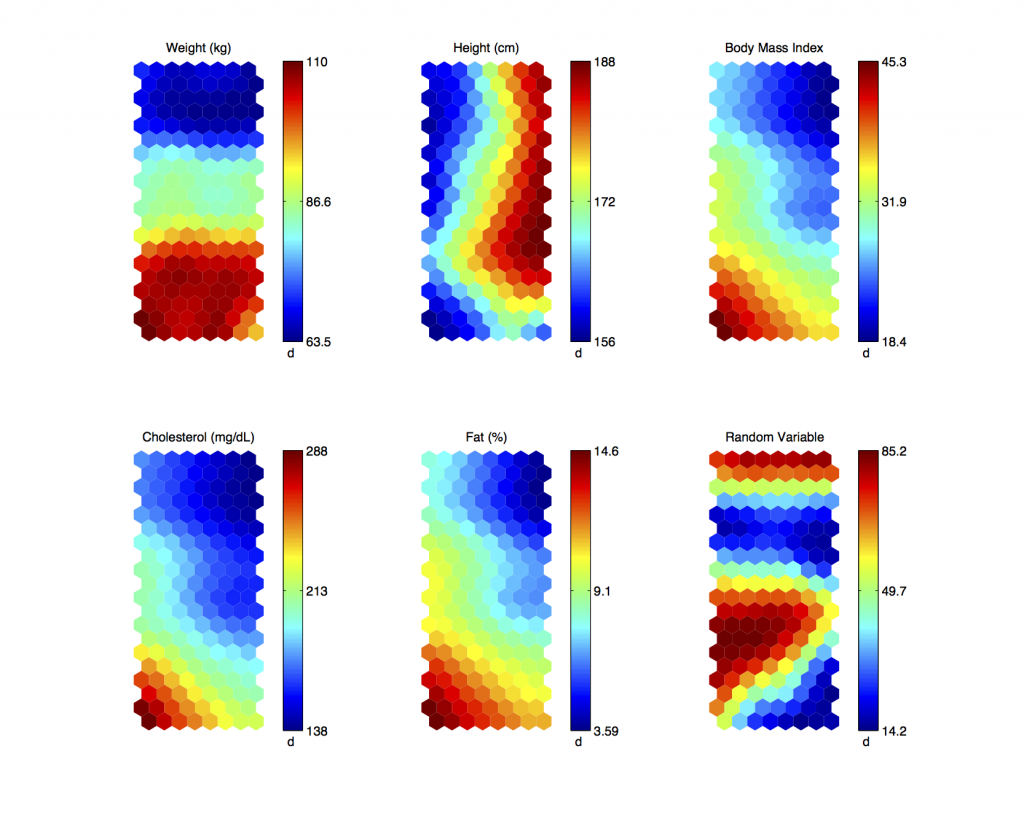
\includegraphics[keepaspectratio,
                                 width=\paperwidth,
                                 height=\paperheight]{kohonen-map.png}
            };
        \end{tikzpicture}
     \end{frame}
}


\begin{frame}[t]
  \frametitle{Достоинства и недостатки карт Кохонена}

   $+$ возможность визуального анализа многомерных данных

   $-$ {\bf Искажения}. Близкие в исходном пространстве могут перейти в далёкие точки на карте, и наоборот.

   $-$ {\bf Субъективность}. Карта зависит не только от кластерной структуры данных, но и от...

   \begin{itemize}
     \item свойств сглаживающего ядра
     \item (случайной) инициализации
     \item (случайного) выбора $x_i$ в ходе итераций
   \end{itemize}

   \vspace{1cm}
   Хорошо подходят для разведочного анализа даннных.
 \end{frame}


\begin{frame}
  \frametitle{Автокодировщики}

  \begin{center}
    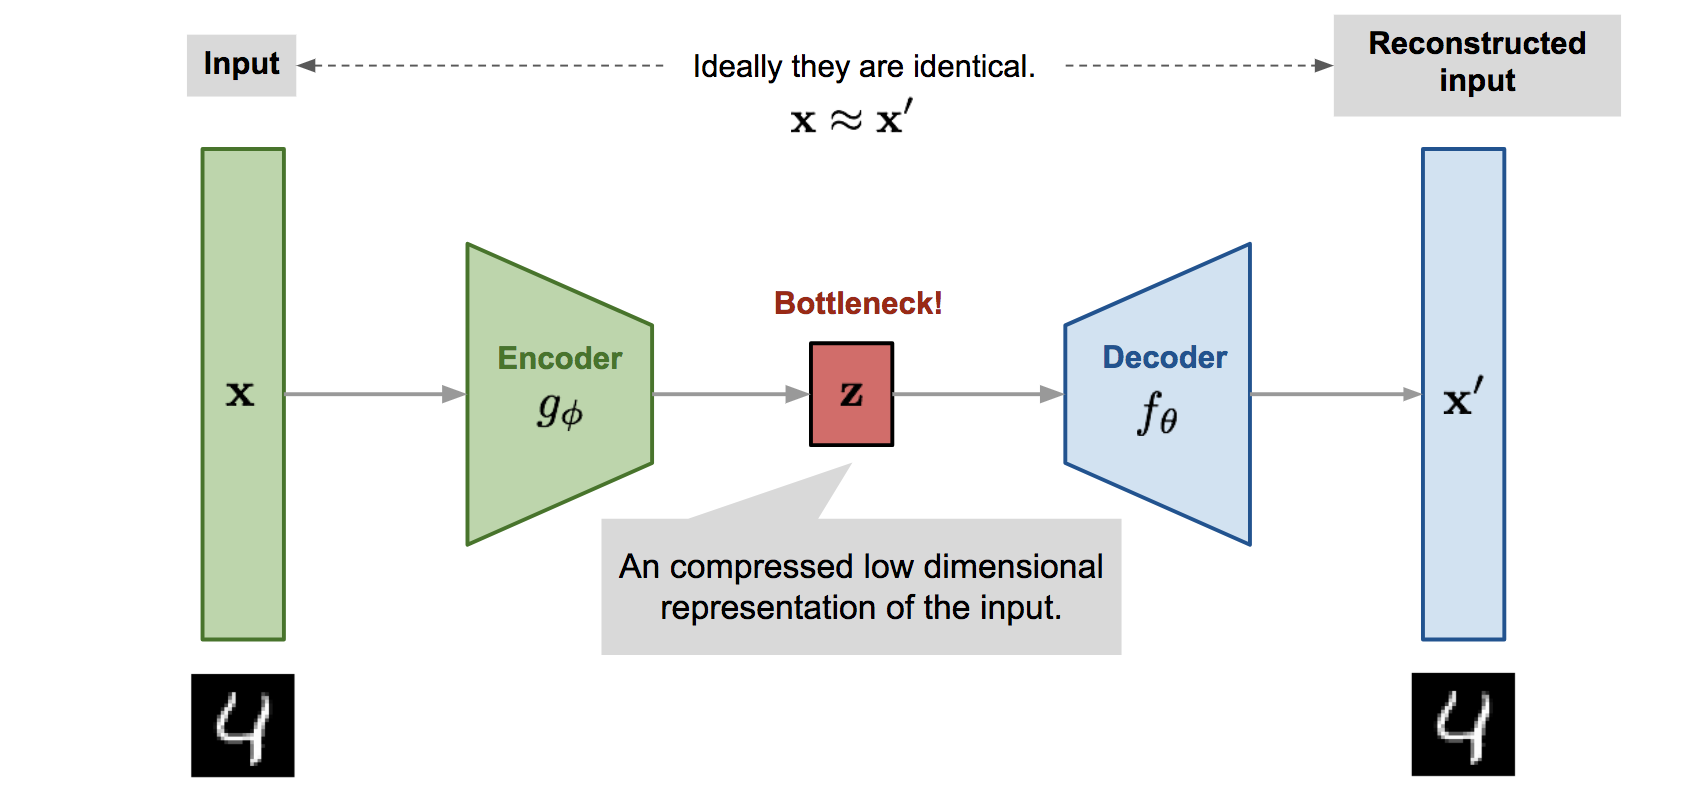
\includegraphics[keepaspectratio,
                     width=0.8\paperwidth]{autoencoder-architecture.png}
  \end{center}
  \pause
  \begin{question}
    Какой метод из первой части курса похож на автокодировщик?
  \end{question}
\end{frame}


\begin{frame}
  \frametitle{Способы использования автокодировщиков}
  \begin{itemize}
    \item Генерация признаков (feature generation), например, для эффективного решения задач обучения с учителем
    \item Снижение размерности (dimensionality reduction)
    \item Сжатие данных с минимальными потерями
    \item Обучаемая векторизация объектов, встраиваемая в более глубокие нейросетевые архитектуры
    \item Генерация синтетических объектов, похожих на реальные
  \end{itemize}

  \noindent\rule{8cm}{0.4pt}

  {\small
  {\it Rumelhart, Hinton, Williams}. Learning Internal Representations by Error Propagation. 1986.

  {\it David Charte et al}. A practical tutorial on autoencoders for nonlinear feature fusion: taxonomy, models, software and guidelines. 2018.}

\end{frame}


\begin{frame}
  \frametitle{Линейный автокодировщик и метод главных компонент}

  $$ \mathscr{L}_{AE}(A, B) = \sum\limits_{i = 1}^\ell \|{\color{red}BA}x_i - x_i \|^2 \to \min\limits_{A,B}$$


  Метод главных компонент:  $F = (x_1\dots x_\ell)^T, U^TU = I_m, G = FU,$

  $$ \|F - GU^T \|^2 = \sum\limits_{i = 1}^\ell \|{\color{red}UU^T}x_i - x_i \|^2 \to \min\limits_{U}$$

  Автокодировщик обобщает метод главных компонент:
  \begin{itemize}
    \item не обязательно $B=A^T$ (хотя часто так делают)
    \item произвольные $A, B$ вместо ортогональных
    \item нелинейные модели
    \item произвольная функция потерь $\mathscr{L}$ вместо квадратичной
    \item SGD оптимизация вместо сингулярного разложения (SVD)
  \end{itemize}
\end{frame}


\begin{frame}
  \frametitle{Разреживающий автокодировщик (Sparse AE)}

  \begin{exampleblock}{Напоминание из SVM}
    Если у функции потерь излом, то отбор объектов. Если в регуляризаторе, то признаков.
  \end{exampleblock}

  \begin{itemize}
    \item Применение $L_1$ или $L_2$-регуляризации к векторам весов
    \item Применение $L_1$-регуляризации к кодовым векторам $z_i = Ax_i$
    \item Энтропийная регуляризация
  \end{itemize}

  \vspace{1cm}
  \noindent\rule{8cm}{0.4pt}

  {\small
  {\it D.Arpit et al}. Why regularized auto-encoders learn sparse representation? 2015}
\end{frame}

\begin{frame}
  \begin{center}
    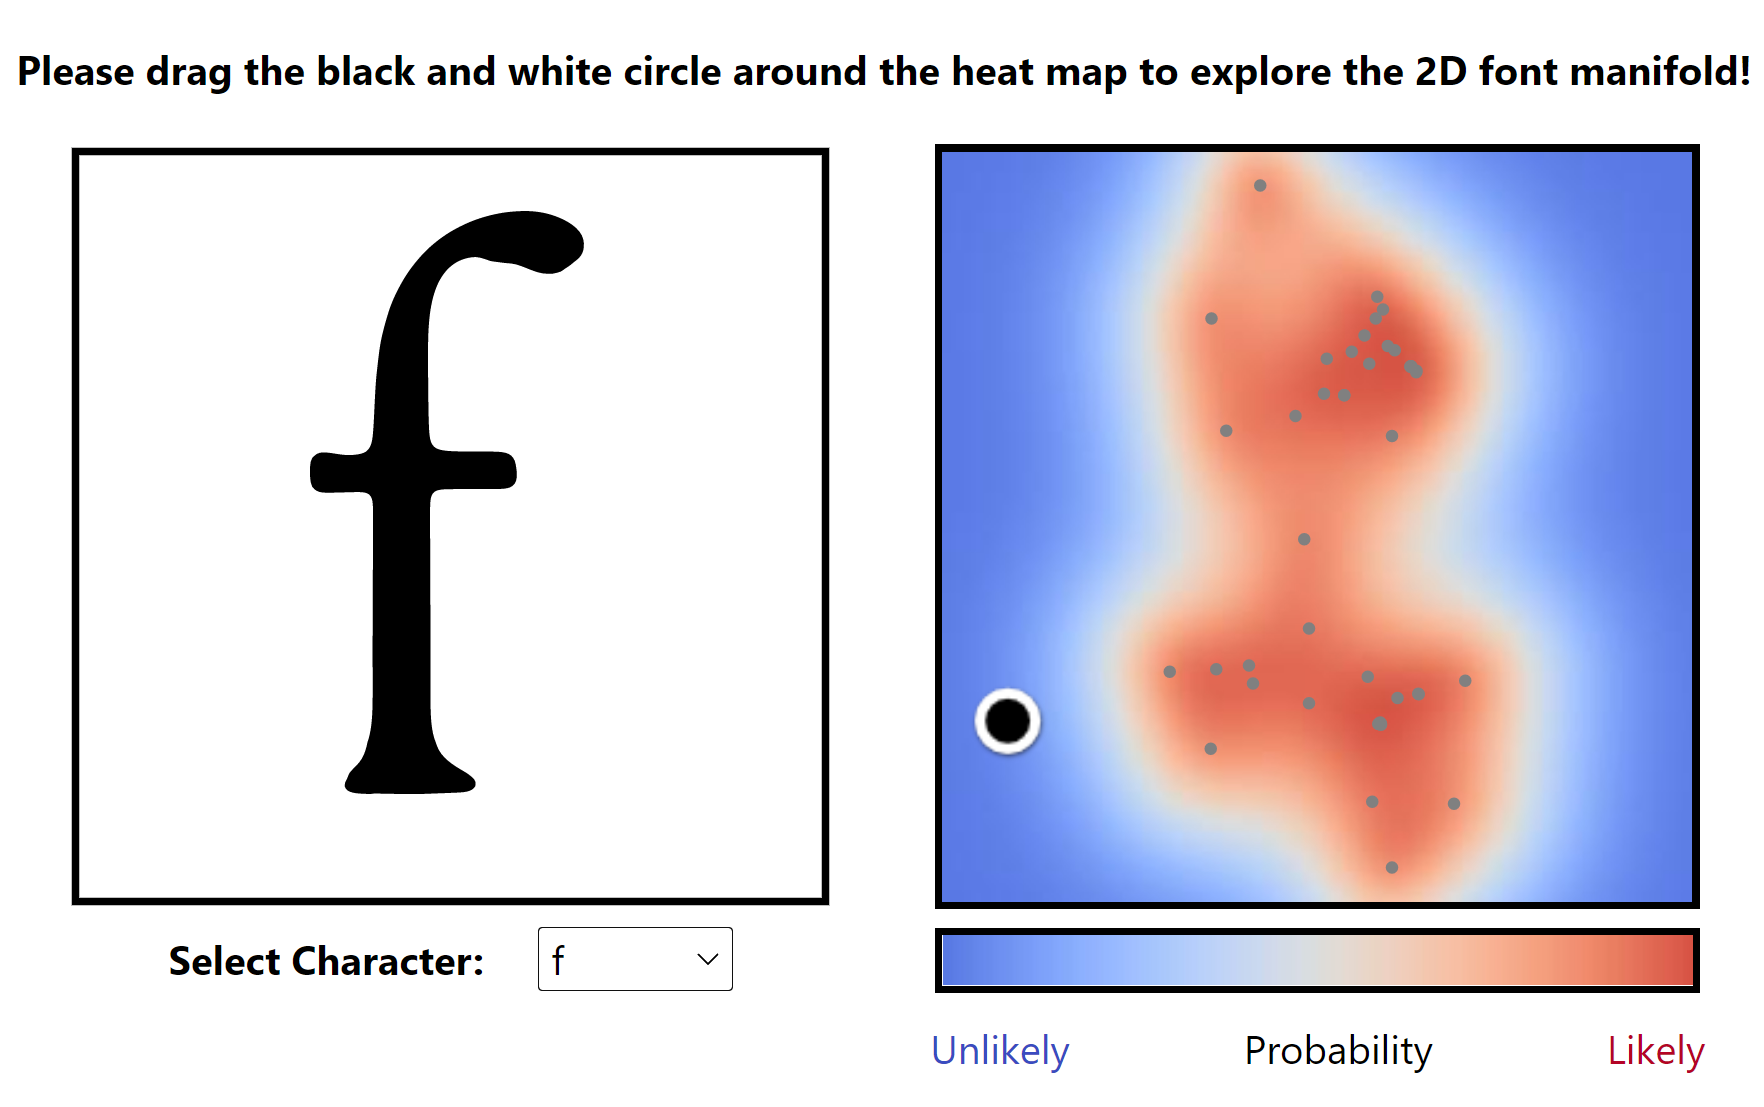
\includegraphics[keepaspectratio,
                     width=0.8\paperwidth]{2d-font-manifold.png}

  \href{https://www.ndfcampbell.org/research/fonts/}{2d font manifold demonstration}
  \end{center}
\end{frame}


\begin{frame}
  \frametitle{Шумоподавляющий автокодировщик (Denoising AE)}

  Устойчивость кодовых векторов $z_i$ относительно шума в $x_i$:

  $$ \mathscr{L}_{DAE}(\alpha, \beta) = \sum\limits_{i = 1}^\ell {\color{red} E_{\tilde x \sim q(\tilde x|x_i)}}
  \mathscr{L}(g(f({\color{red}\tilde x}, \alpha), \beta),x_i) \to \min\limits_{\alpha, \beta}$$

  \begin{columns}
      \begin{column}{.6\paperwidth}
        Вместо вычисления матожидания $E_{\tilde x}$ в методе стохастического градиента объекты $x_i$ сэмплируются и зашумляются по одному: $\tilde x \sim q(\tilde x|x_i)$
        \begin{itemize}
          \item гауссовский шум: $\tilde x \sim N(x_i, \sigma^2 I)$
          \item обнуление компонент вектора $x_i$ с вероятностью $p_0$
        \end{itemize}
      \end{column}
      \begin{column}{.3\paperwidth}
        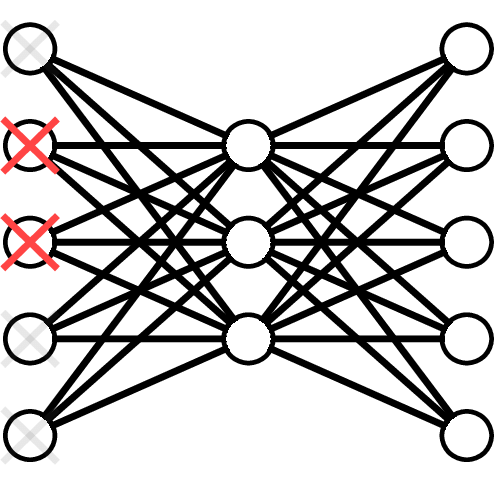
\includegraphics[keepaspectratio,
                       width=.3\paperwidth]{denoising-AE.png}
      \end{column}
  \end{columns}

  \noindent\rule{8cm}{0.4pt}

  {\small
  {\it P. Vincent, H. Larochelle, Y. Bengio, P.-A. Manzagol}. Extracting and composing robust features with denoising autoencoders. ICML-2008.}
\end{frame}


\begin{frame}
  \frametitle{Вариационный автокодировщик (Variational AE)}

  Строится генеративная модель, способная порождать новые объекты $x$, похожие на объекты выборки $X^\ell = \{x_1,\dots,x_\ell \}$

  $q_\alpha(z|x)$ — вероятностный кодировщик с параметром $\alpha$

  $p_\beta(\hat x|z)$ — вероятностный декодировщик с параметром $\beta$

  \begin{align*}
    \mathscr{L}_{VAE}(\alpha, \beta) = \sum\limits_{i=1}^\ell \log p(x_i) = \sum\limits_{i=1}^\ell \log \int q_{\alpha} (z | x_i) \frac{p_{\beta}(x_i|z) p(z)}{q_{\alpha} (z | x_i)} dz \geq \\
    \geq \sum\limits_{i=1}^\ell \int q_\alpha(z|x_i) \log p_\beta(x_i|z)dz - KL(q_\alpha(z|x_i)\| p(z)) \to \max\limits_{\alpha, \beta}
  \end{align*}

  \noindent\rule{8cm}{0.4pt}

  {\small
  {\it D.P.Kingma, M.Welling.} Auto-encoding Variational Bayes. 2013.

  {\it C.Doersch.} Tutorial on variational autoencoders. 2016.}
\end{frame}


\begin{frame}

$$ \sum\limits_{i=1}^\ell \underbrace{E_{z \sim q_{\alpha}(z|x_i)} \log p_\beta(x_i|z)}_{\text{качество реконструкции}} -
\underbrace{KL(q_\alpha(z|x_i)\| p(z))}_{
  \text{регуляризатор по } \alpha
}
\to \max\limits_{\alpha, \beta}$$

где $p(z)$ — априорное распределение, обычно $N(0, \sigma^2 I)$
\pause
\vspace{0.5cm}
{\bf Репараметризация} $q_\alpha (z|x_i):\ z = f(x_i, \alpha, \varepsilon),\ \varepsilon \sim N(0, I)$

\vspace{0.5cm}{\bf Метод стохастического градиента}:
\begin{itemize}
  \item сэмплировать $x_i \sim X^\ell,\ \varepsilon \sim N(0, I),\ z = f(x_i, \alpha, \varepsilon)$
  \item градиентный шаг
  $ \alpha = \alpha + h \nabla_\alpha[\log p_\beta(x_i|f(x_i, \alpha, \varepsilon)) - KL(q_\alpha(z|x_i)\| p(z))] $

  $ \beta = \beta + h \nabla_\beta[\log p_\beta(x_i|z)] $
\end{itemize}


\vspace{0.5cm}
{\bf Генерация похожих объектов}: $$x \sim p_\beta(x|f({\color{red}x_i}, \alpha, \varepsilon)), \varepsilon \sim N(0, I)$$
\end{frame}


\begin{frame}
  \frametitle{Автокодировщики для обучения с учителем}

  {\bf Данные:} неразмеченные $(x_i)_{i=1}^\ell$, размеченные $(x_i, y_i)_{i=\ell+1}^{\ell + k}$

  \vspace{0.5cm}
  {\bf Совместное обучение} кодировщика, декодировщика и предсказательной модели (классификации, регрессии или др.)

  $ \sum\limits_{i=1}^\ell \mathscr{L}(g(f(x_i, \alpha), \beta), x_i)
  + \lambda \sum\limits_{i=\ell+1}^{\ell+k} \tilde{\mathscr{L}}(\hat y(f(x_i, \alpha), \gamma), y_i) \to \min\limits_{\alpha, \beta, \gamma}$

  \vspace{0.5cm}
  {\bf Функции потерь:}

  $\mathscr{L}(\hat x_i, x_i)$ — реконструкция

  $\tilde{\mathscr{L}}(\hat y_i, y_i)$ — предсказание

  \vspace{1cm}

  \noindent\rule{8cm}{0.4pt}

  {\small
  {\it Dor Bank, Noam Koenigstein, Raja Giryes.} Autoencoders. 2020.}
\end{frame}

\begin{frame}
  \begin{align*}
      z_i &= f(x_i, {\color{blue}\alpha}) \text{ — кодировщик} \\
      \hat x_i &= g(z_i, {\color{green}\beta}) \text{ — декодировщик} \\
      \hat y_i &= \hat y(z_i, {\color{orange}\gamma}) \text{ — классификатор}
  \end{align*}
  \begin{center}
    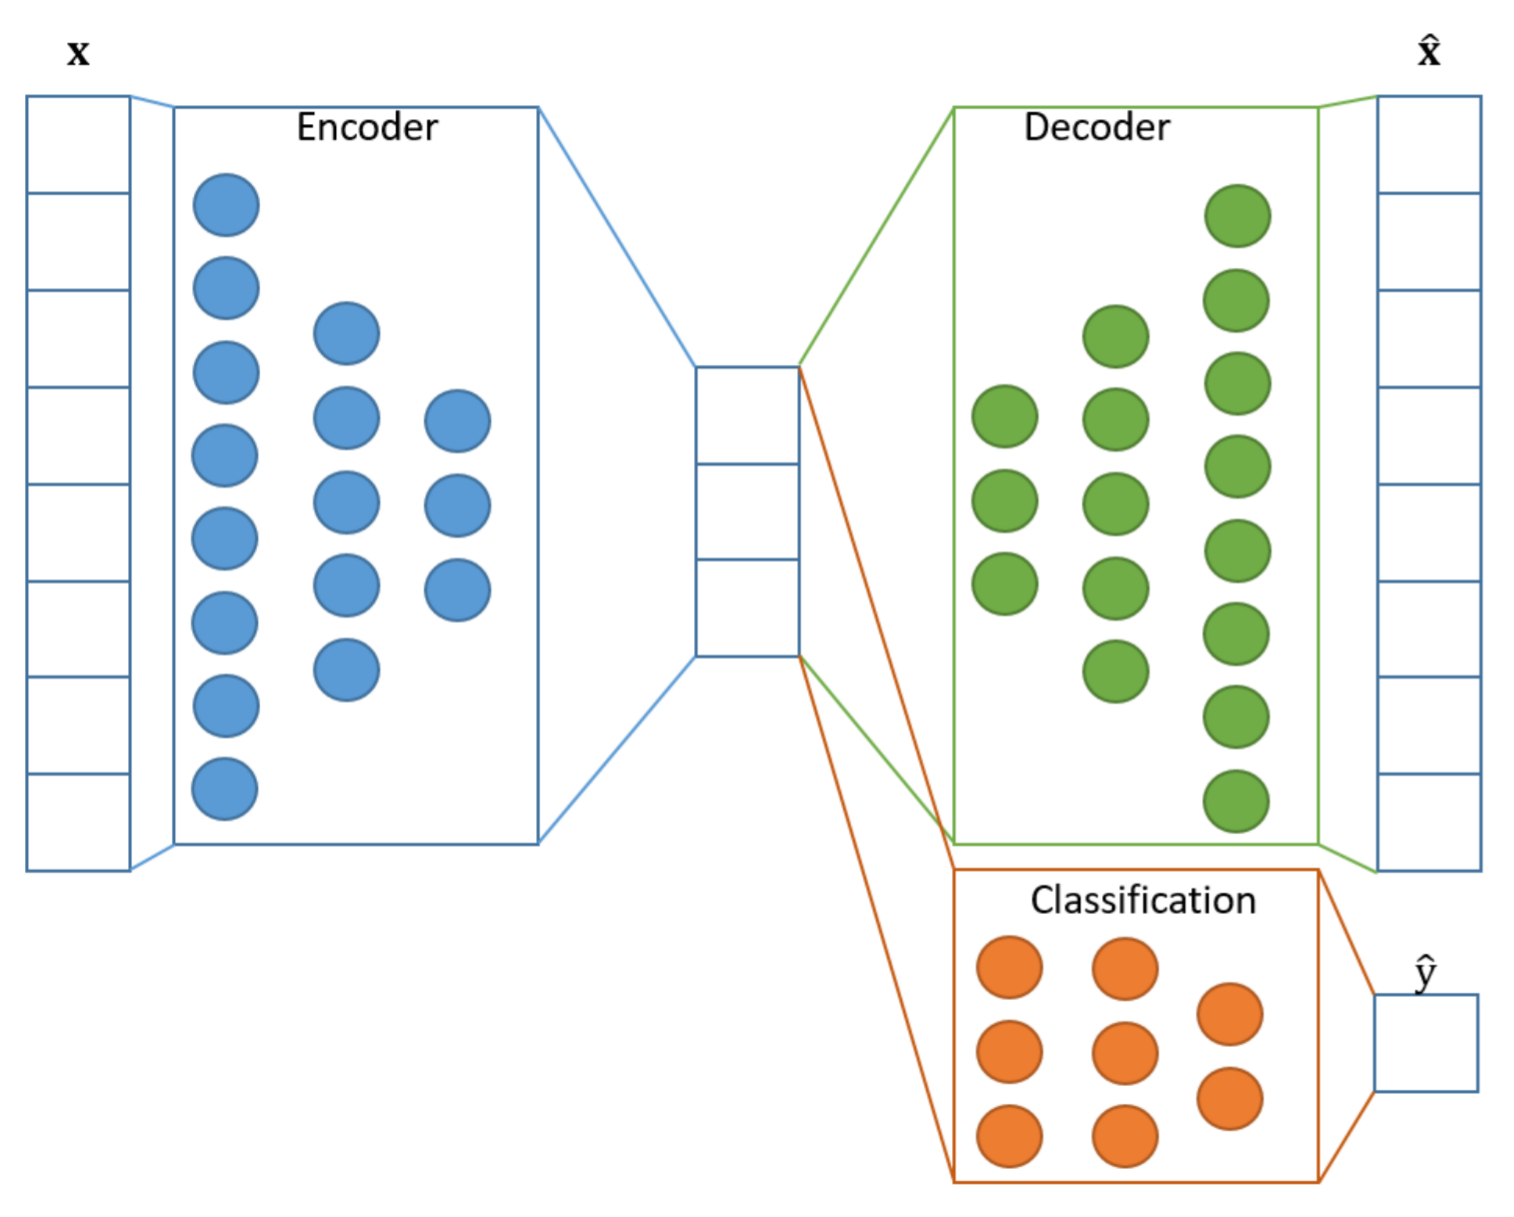
\includegraphics[keepaspectratio,
                   width=.6\paperwidth]{autoenc_supervised.png}
  \end{center}
\end{frame}


\begin{frame}
  \frametitle{Пред-обучение нейронных сетей (pre-training)}

  Свёрточная сеть для обработки изображений:

  \begin{itemize}
    \item $\color{red}{z=f(x,\alpha)}$ — свёрточные слои для векторизации объектов
    \item $y = g(z, \beta)$ — полносвязные слои под конкретную задачу
  \end{itemize}

  \begin{center}
    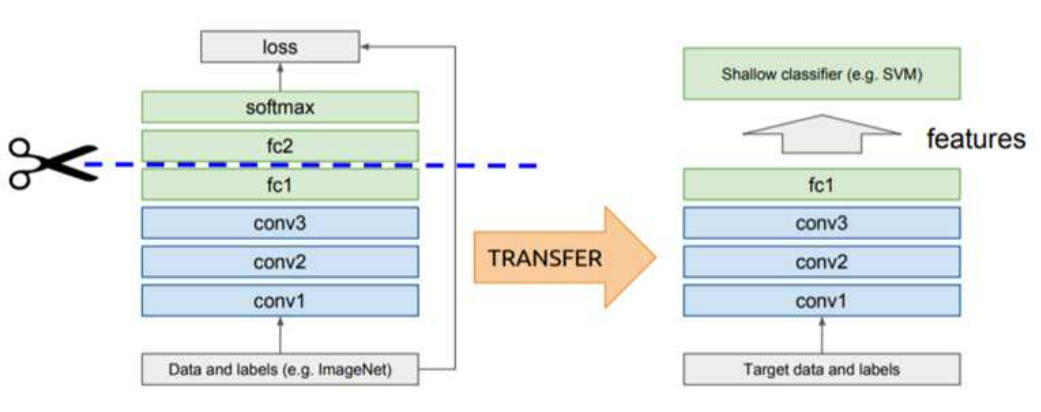
\includegraphics[keepaspectratio,
                   width=.8\paperwidth]{pre-training.png}
  \end{center}

  \noindent\rule{8cm}{0.4pt}

  {\small
  {\it Jason Yosinski, Jeff Clune, Yoshua Bengio, Hod Lipson.} How transferable are features in deep neural networks? 2014.}
\end{frame}


\begin{frame}
  \frametitle{Перенос обучения (transfer learning)}

  \begin{itemize}
    \item ${\color{red}f(x,\alpha)}$ — универсальная часть модели (векторизация)
    \item $g(x, \beta)$ — специфичная для задачи часть модели
  \end{itemize}

  {\it Базовая задача} на выборке $\{x_i\}_{i=1}^\ell$ с функцией потерь $\mathscr{L}_i$:

  $$\sum\limits_{i=1}^\ell \mathscr{L}_i ({\color{red}f(x_i,\alpha)}, g(x_i, \beta)) \to \min_{\alpha, \beta} $$

  {\it Целевая задача} на другой выборке $\{x_i^\prime\}_{i=1}^m$ с другими $\mathscr{L}_i^\prime, g^\prime$:

  $$\sum\limits_{i=1}^m \mathscr{L}_i^\prime ({\color{red}f(x_i^\prime,\alpha)}, g^\prime(x_i^\prime, \beta^\prime)) \to \min_{ \beta^\prime} $$

  при $m \ll \ell$ это может быть намного лучше, чем

  $$\sum\limits_{i=1}^m \mathscr{L}_i^\prime (f(x_i^\prime,\alpha), g^\prime(x_i^\prime, \beta^\prime)) \to \min_{\alpha, \beta^\prime} $$

  \noindent\rule{8cm}{0.4pt}

  {\small
  {\it Sinno Jialin Pan, Qiang Yang.} A Survey on Transfer Learning. 2009}
\end{frame}


\begin{frame}
  \frametitle{Многозадачное обучение (multi-task learning)}

  \begin{itemize}
    \item ${\color{red}f(x,\alpha)}$ — универсальная часть модели (векторизация)
    \item $g(x, \beta)$ — специфичные части модели для задач $t \in T$
  \end{itemize}

  Одновременное обучение модели $f$ по задачам $X_t, t \in T$:

  \begin{center}
  $\sum\limits_{t \in T} \sum\limits_{i \in X_t} \mathscr{L}_{ti} ({\color{red}f(x_{ti},\alpha)}, g(x_{ti}, \beta_t)) \to \min_{\alpha, \{\beta_t\}} $
  \end{center}

  \vspace{0.2cm}
  Обучаемость (learnability): качество решения отдельной задачи $\left< X_t, \mathscr{L}_t, g_t\right>$
  улучшается с ростом объёма выборки $\ell_t = |X_T|$.

  \vspace{0.2cm}
  Learning to learn: качество решения каждой из задач $t \in T$ улучшается с ростом $\ell_t$ и общего числа задач $|T|$.

  \vspace{0.2cm}
  Few-shot learning: для решения задачи $t$ достаточно небольшого числа примеров, иногда даже одного.

  \noindent\rule{8cm}{0.4pt}

  {\tiny
  {\it M.Crawshaw.} Multi-task learning with deep neural networks: a survey. 2020

  {\it Y.Wang et al.} Generalizing from a few examples: a survey on few-shot learning. 2020}
\end{frame}


\begin{frame}
  \frametitle{Самостоятельное обучение (self-supervised learning)}

  Модель векторизации ${\color{red}z=f(x,\alpha)}$ обучается предсказывать взаимное расположение пар фрагментов одного изображения

  \begin{center}
    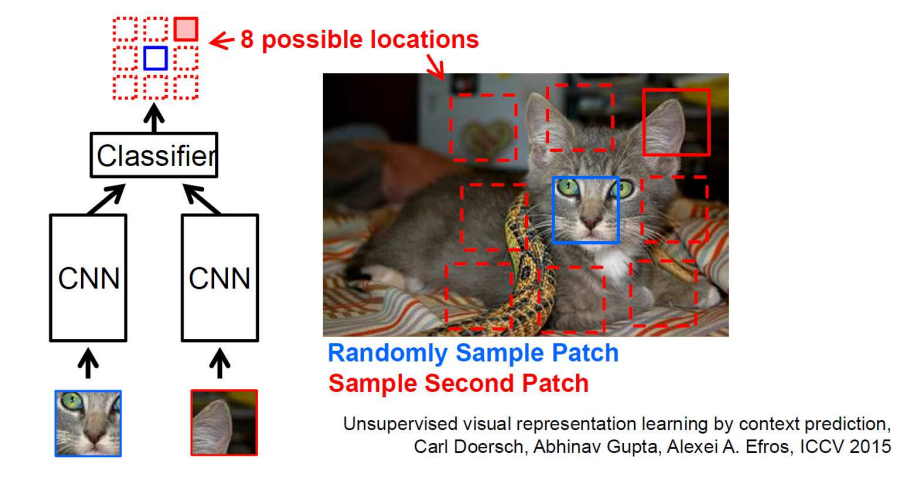
\includegraphics[keepaspectratio,
                     width=.7\paperwidth]{self-supervised.png}
  \end{center}

  {\bf Преимущество:} сеть выучивает векторные представления объектов без размеченной обучающей выборки. Их качество не уступает полученным по размеченному ImageNet.
\end{frame}


\begin{frame}
  \frametitle{Дистилляция моделей или суррогатное моделирование}

  Обучение ${\color{red}\text{сложной модели } a(x, w)}$ «долгое, дорогое»:
  $$\sum\limits_{i=1}^\ell \mathscr{L}(\color{red}{a(x_i, w)}, y_i) \to \min_{w} $$
  Обучение ${\text{простой модели } b(x, w^\prime)}$, возможно, на других данных:
  $$\sum\limits_{i=1}^k \mathscr{L}({b(x_i^\prime, w^\prime)}, {\color{red}a(x_i^\prime, w)}) \to \min_{w^\prime} $$
  {\bf Примеры задач:}
  \begin{itemize}
    \item замена сложной модели (климат, аэродинамика и др.), которая вычисляется на суперкомпьютере месяцами, <<лёгкой>> аппроксимирующей суррогатной моделью
    \item замена сложной нейросети, которая обучается неделями на больших данных, <<лёгкой>> аппроксимирующей нейросетью с минимизацией числа нейронов и связей
    \end{itemize}
\end{frame}

\begin{frame}
  \frametitle{Обучение с использованием привилегированной информации}

  LUPI — Learning Using Priveleged Information

  \begin{center}
    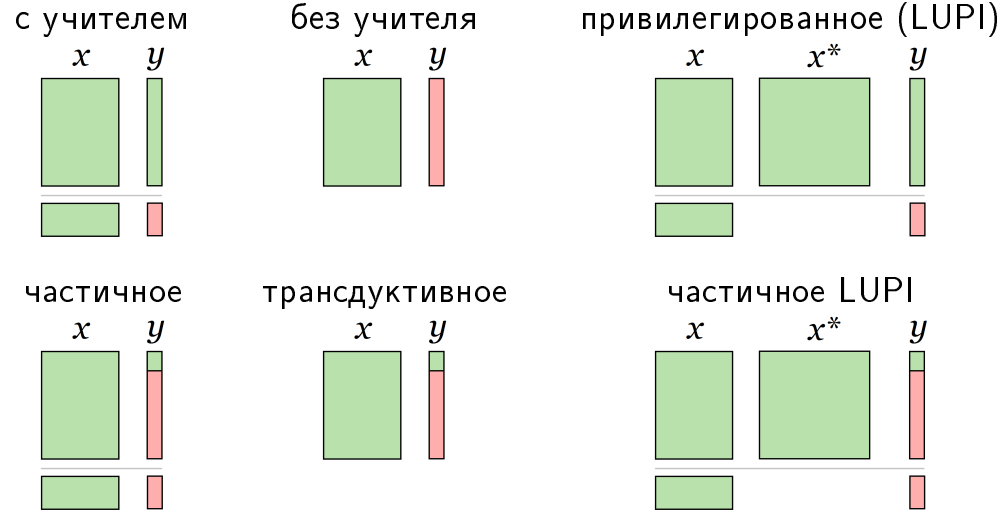
\includegraphics[keepaspectratio,
                     width=.7\paperwidth]{LUPI.png}
  \end{center}

  \noindent\rule{8cm}{0.4pt}

  {\small
  {\it V.Vapnik, A.Vashist.} A new learning paradigm: Learning Using Privileged Information // Neural Networks. 2009.}
\end{frame}


\begin{frame}
  \frametitle{Примеры задач с привилегированной информацией $x^*$}
  \begin{itemize}
    \item $x$ — первичная (1D) структура белка

          $x^*$ — третичная (3D) структура белка

          $y$ — иерархическая классификация функции белка
    \item $x$ — предыстория временного ряда

          $x^*$ — информация о будущем поведении ряда

          $y$ — прогноз следующей точки ряда
    \item $x$ — текстовый документ

          $x^*$ — выделенные ключевые слова или фразы

          $y$ — категория документа
    \item $x$ — пара (запрос, документ)

          $x^*$ — выделенные асессором ключевые слова или фразы

          $y$ — оценка релевантности
  \end{itemize}
\end{frame}

\begin{frame}
  \frametitle{Задача обучения с привилегированной информацией}

  \begin{itemize}
    \item Раздельное обучение модели-ученика и {\color{red} модели-учителя}:

    $\sum\limits_{i=1}^\ell \mathscr{L}(a(x_i, w), y_i) \to \min_{w} \quad\quad
    \sum\limits_{i=1}^\ell \mathscr{L}({\color{red}a(x_i^*, w^*)}, y_i) \to \min_{w} $

    \item Модель-ученик обучается повторять ошибки {\color{red} модели-учителя}:

    $\sum\limits_{i=1}^\ell \mathscr{L}(a(x_i, w), y_i) + \mu
     \mathscr{L}(a(x_i, w), {\color{red}a(x_i^*, w^*)}) \to \min_{w} $

    \item {\bf Совместное обучение} модели-ученика и {\color{red} модели-учителя}:

    $\sum\limits_{i=1}^\ell \mathscr{L}(a(x_i, w), y_i) + \lambda \mathscr{L}({\color{red}a(x_i^*, w^*)}, y_i)
    + \mu \mathscr{L}(a(x_i, w), {\color{red}a(x_i^*, w^*)}) \to \min_{w, w^*}$
  \end{itemize}

  \noindent\rule{8cm}{0.4pt}

  {\small
  {\it D.Lopez-Paz, L.Bottou, B.Scholkopf, V.Vapnik.} Unifying distillation and privileged information. 2016.}
\end{frame}


\begin{frame}
  \frametitle{Генеративная состязательная сеть (Generative Adversarial Net, GAN)}

  Генератор $G(z)$ учится порождать объекты $x$ из шума $z$

  Дискриминатор $D(x)$ учится отличать их от реальных объектов

  \begin{center}
    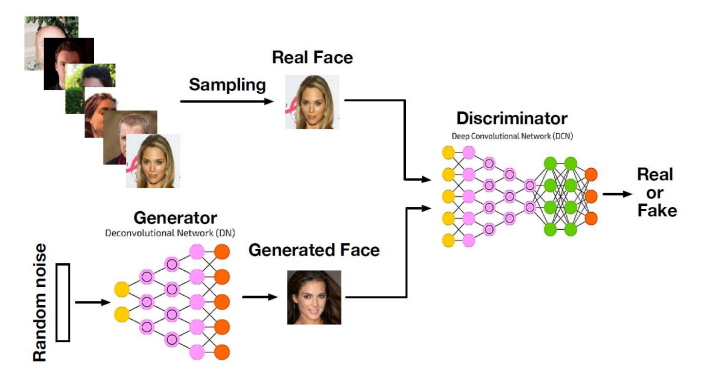
\includegraphics[keepaspectratio,
                     width=.7\paperwidth]{GAN_scheme.png}
  \end{center}

  \noindent\rule{8cm}{0.4pt}

  {\tiny
  {\it Antonia Creswell et al.} Generative Adversarial Networks: an overview. 2017.

  {\it Zhengwei Wang, Qi She, Tomas Ward.} Generative Adversarial Networks: a survey and taxonomy. 2019.

  {\it Chris Nicholson.} \href{https://pathmind.com/wiki/generative-adversarial-network-gan}{A Beginner's Guide to Generative Adversarial Networks}. 2019.
  }
\end{frame}


\begin{frame}
  \frametitle{Постановка задачи GAN}

  Есть выборка объектов $\{x_i\}_{i=1}^m$ из $X$

  Обучаем

  \begin{itemize}
    \item вероятностную генеративную модель $G(z, \alpha): x \sim p(x|z,\alpha)$
    \item вероятностную дискриминативную модель $D(x, \beta) = p(1| x, \beta)$
  \end{itemize}

  {\bf Критерии}:
  \begin{itemize}
    \item обучение дискриминативной модели $D$:
      $$ \sum\limits_{i=1}^m \ln D(x_i, {\color{red}\beta}) + \ln(1 - D(G(z_i, \alpha), {\color{red}\beta})) \to {\color{red}\max\limits_{\beta}}$$
    \item обучение генеративной модели $G$ по случайному шуму $\{z_i\}_{i=1}^m$:
      $$ \sum\limits_{i=1}^m \ln(1 - D(G(z_i, {\color{red}\alpha}), \beta)) \to {\color{red}\min\limits_{\alpha}}$$
  \end{itemize}

  \noindent\rule{8cm}{0.4pt}

  {\small
  {\it Ian Goodfellow et al.} Generative Adversarial Nets. 2014}
\end{frame}


\begin{frame}
  \frametitle{StyleGAN demo}

  \href{https://www.youtube.com/watch?v=kSLJriaOumA}{Посмотрим видео}

  \vspace{2cm}
  Cтатьи тут: \href{https://nvlabs.github.io/stylegan2/versions.html}{https://nvlabs.github.io/stylegan2/versions.html}

\end{frame}

\begin{frame}
  \frametitle{Резюме}
  \begin{itemize}
    \item Кластеризация и карты Кохонена
    \item Автокодировщики, включая совместное обучение с классификацией
    \item Многозадачное обучение (multi-task learning)
    \item Перенос обучения (transfer learning)
    \item Дистилляция и суррогатное моделирование
    \item Состязательные сети (GAN)
  \end{itemize}
  \pause
  \vspace{1cm}
  Что ещё можно посмотреть?
  \begin{itemize}
    \item \href{https://www.youtube.com/watch?v=5WoItGTWV54}{Лекцию 13} курса CS231n про GAN
  \end{itemize}
\end{frame}

\end{document}
